\newpage
% These: Google Street View sollte in Deutschland erweitert und aktualisiert werden.
% Hauptteil:
%   - Argumentation der Kernaussagen
%   - Transferleistung
%   - Ableitung und Begründung eigener Position

% Pro:
% - Help find way (especially with AR when walking)
% 
% Contra:
% - Opt-in vs. Opt-out
% - Welche Daten werden wirklich erhoben
% - Debakel mit WLAN Scanning
% - 

\section{Hauptteil}\label{hauptteil}

\subsection{Google Street View im Detail}\label{street-view-detail}
% - Wie funktioniert GSV?
%   - Autos mit Panorama
%     - https://www.google.com/intl/de/streetview/explore/
%   - Sehr gutes GPS mit anderen Sensoren
%     - https://www.trekview.org/blog/2019/google-street-view-cameras-more-than-meets-the-eye/
Um die 360\degree\ Panoramen aufzunehmen nutzt Google Fahrzeuge, die durch die
aufzunehmenden Straßen fahren (Siehe Abb. \ref{fig:gsv-car}).

\begin{wrapfigure}{r}{0.4\textwidth}
  \caption{Google Street View Fahrzeug}\label{fig:gsv-car}
  \begin{center}
    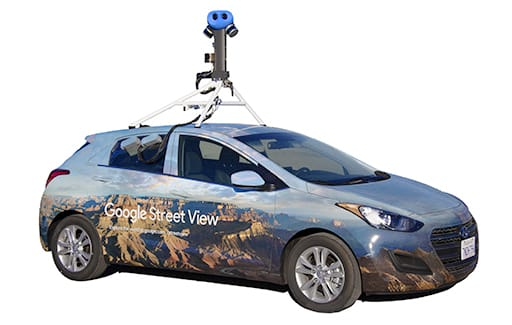
\includegraphics[width=\textwidth]{gsv-car}
    \\
    \cite[Quelle:][]{website:google-street-view:about}
  \end{center}
\end{wrapfigure}


Nachdem das Fahrzeug die Bilder aufgenommen hat, folgt die Nachbearbeitung. Hier
werden die einzelnen Bilder der Linsen in ein 360\degree\ Panorama zusammengestellt,
die Kennzeichen von anderen Fahrzeugen und die Gesichter von Personen verpixelt
und einige manuelle Nacharbeiten erledigt. Durch diesen Prozess dauert es von wenigen
Wochen bis zu mehreren Monaten bis die aufgenommenen Bilder in Goolge Street
View der Allgemeinheit verfügbar gemacht werden.

Neben den Kameras haben die Street View Fahrzeuge auch noch andere Sensoren:
beispielsweise ein genaues GPS-System, Messgeräte für Abstand, Tiefe und
Luftqualität. Zwischen 2008 und 2010 waren die Fahrzeuge auch mit einem WLAN
Scanner ausgestattet, das die Namen und MAC Addressen von Routern aufgezeichnet
hat, um die Positionierung in Android Smartphones zu verbessern.\footcite{website:trekview:gsv-sensors}

\subsection{Welche Daten kann man aus Google Street View erlangen}

In diesem Abschnitt wird gezeigt, wie die oben beschriebenen Daten von Google
und auch von allen anderen genutzt werden oder werden können, um einen Einblick
in die Möglichkeiten und die Implikationen für die Privatsphäre abzuschätzen

\subsubsection{WLAN Scanning}

Durch das WLAN Scanning hat Google folgende Daten erlangen können:

\begin{enumerate}
  \item Name und MAC Addresse des WLAN Routers oder Access Points \label{name-and-mac}
  \item Stärke des WLAN Signals an der jeweiligen Position \label{signal-strength}
  \item Netzwerkverkehr von ungesicherten WLAN Netzwerken \label{network-traffic}
\end{enumerate}

Durch die Punkte \ref{name-and-mac} und \label{signal-strength} ist es für
Google möglich, eine genauere Positionierung als GPS alleine anzubieten. Diese
Datensammlung ermöglicht Google eine Positionsbestimmung obwohl kein GPS Signal
erfangen werden kann; besonders in dichten Städten, in denen GPS Signale häufig
durch die hohen Häuser eingeschränkt sind und viele WLANs von den Häusern
ausgehen. Der Dienst der genauren Positionsbestimung findet anwendungs in Google
Smartphonebetriebssystem Android und der Google Maps App (unabhängig vom
Betriebssystem).

Im Gegensatz dazu steht der Punkt \ref{network-traffic}, der laut Google aus
Versehen gesammelt wurde. Die Daten würden von Google nicht genutzt werden.
Ebenso argumentiert Google, dass die Daten unvollständig sind, weil sich die
Fahrzeuge bewegen und der WLAN Channel fünfmal pro Sekunde gewechselt wird.\footcite{website:googleblog:wifi-data-collection}

Trotzdem wurde Google für diese Datensammlung sanktioniert. Die Daten mussten in
einigen Ländern gelöscht werden\footcite{website:isec:ireland-destroy-notice}, in
Deutschland gab es am 22.04.2013 wurde ein Bußgeld in Höhe von 145 000 EUR von dem
Hamburger Datenschutzbeauftragten Johannes Caspar verhängt\footcite{website:nwzonline:google-wifi-sanction}
und in den USA wurde vom Attorney General ein Bußgeld in Höhe von 7 Mio. USD verhängt.%\footnote{https://portal.ct.gov/AG/Press-Releases-Archived/2013-Press-Releases/Attorney-General-Announces-7-Million-Multistate-Settlement-With-Google-Over-Street-View-Collection-o}

\subsubsection{Fotos}

Die Daten aus dem WLAN Scanning sind nicht für alle verefügbar. Es werde auf der
Website und der mobilen App nur die 360\degree\ Panoramen bereitgestellt. Es ist
also interessant zu sehen, welche Daten man aus diesen Bildern extrahieren kann.

Die offentlichlichsten personenbezogenen Daten - Gesichter und Kennzeichen -
werden bereits automatisch verpixelt. Danach wird es durch Google Mitarbeiter
noch einmal validiert, dass diese Merkmale wirklich verpixelt wurden. Falls
dieser Prozess noch immer nicht alles verpixelt hat, bietet Google die
Möglichkeit ein Panorama zu melden, damit es noch einmal für eine manuelle
Sichtung und Nachbesserung markiert wird.

Es gibt aber durchaus andere Daten, die nicht für jeden ersichtlich sein sollen.
Bilder eines Einganges zu einer Basis der Britische Spezialeinheit SAS (Special
Air Services) haben dazu geführt, dass das MoD (Ministery of Defense) zur
Löschung der Bilder auffordert\footcite{website:bbc:herefordshire}. Ebenso ergab
sich ähnliches in den USA\footcite{website:reuters:pentagon-takedown-notice}.

Wissenschaftler\_innen nutzen Google Street View als Datengrundlage für eine
weitreichende Datenanalyse im Bereich Big Data und Machine Learning. Folgende
Themen und Werke werden als Beispiele näher beschrieben:

\begin{enumerate}
  \item Zur Planung von 5G Masten - \cite{Zhang_2020}\label{5g}
  \item Das Volumen an Fußgängern - \cite{YIN2015337}\label{pedestrian-volume}
  \item Die Demographie der Nachbarschaft - \cite{Gebru13108}\label{demographics}
  \item Die Wahrscheinlichkeit für einen Autounfall eines Bewohners - \cite{kita2019google}\label{car-accident}
  \item Die Gesundheit von Bewohnern einer bestimmten
  Nachbarschaft - \cite{8933431} und \cite{DBLP:journals/corr/abs-1905-06464}\label{health}
\end{enumerate}

In Arbeit \ref{5g} werden die Bilder von Google Street View genutzt, um
herauszufunden, wo sich Straßenbeleuchtungsmasten befinden. Es wird dadurch
möglich Masten für den neuen Funkstandard 5G zu planen, weil diese relativ
günstig an vorhandener Straßenbeleuchtung angebracht werden können.

Arbeit \ref{pedestrian-volume} misst das Volumen an Fußgängern, die zu der
Aufnahme der Google Street View Bilder draußen waren. Diese Daten können dann
genutzt werden, um zu urteilen, wie aktiv Menschen in einer Umgebung sind und
was Menschen dazu bringt mehr Zeit draußen zu verbringen. Weitere Informationen
über den Zusammenhang von Stadtbidl und physikalischer Aktivität findet man in
den Forschungsarbeiten vbon Li Yin an der State University of New York.

In Punkt \ref{demographics} wird gezeigt, dass die Google Street View Bilder
ebenso genutzt werden können, um Aussagen über die Nachbarschaft oder Region zu
treffen. In dieser Arbeit werden die fotografierten Autos (Marke, Modell und
Jahr) als Proxy für Demographie genutzt. Die Arbeit zeigt, dass wenn die Anzahl
der fahrenden Sedans höher ist als die Anzahl der Pickup Trucks, die Stadt
wahrscheinlich für die Demokraten stimmen wird. Eben falls konnten Einkommen,
Hautfarbe und Bildung aufgrund dieser Daten bestimmt werden.
% Die Arbeit von M. De Nadai et al. findet einen Zusammenhang zwischen
% der physikalischen Aktivität und der "Sicherheit" der Nachbarschaft. Die Daten
% über die "Sicherheit" kommen aus dem Place Pulse 2.0 Datensatz, in dem Menschen
% zwei Bilder von Häuserfronten und Straßen gezeigt wurde und diese urteilen
% mussten, welches Bild sicherer aussieht. Aus der Arbeit wird ähnlich wie bei
% \ref{pedestrian-volume} herausgearbeitet, welche Eigenschaften von Bildern
% besonders sicher aussehen.

Die Arbeit \ref{car-accident} beschreibt wie Bilder von Google Street View
besseren Aufschluss über die Wahrscheinlichkeit eines Autounfalls geben kann,
als andere Risikomodellen (beispielsweise basierend auf Alter, Postleitzahl),
die von Versicherungen genutzt werden. Diese Daten, argumentieren die Autoren,
können später auch von den Banken genutzt werden, da in anderen Arbeiten gezeigt
wurde, dass die Kreditwürdigkeit und Risikobewertung von Versicherungen
zusammenhängen\footcite{doi:10.1080/10920277.2016.1209118}.

Im Punkt \ref{health} ist zu sehen, dass die Bilder, die aus Google Street View
einzusehen sind, auch dafür genutzt werden können, um Aussagen über die
Gesundheit der Bewohner zu treffen. Solche Daten sind interessant für
Stadplaner, die überprüfen können, ob man etwas an der Umgebung ändern kann, was
die Bewohner anregt sich zu bewegen. Ebenfalls sind die Daten für
Krankenversicherungen interessant, um das Risiko von Krankheiten genauer abzuschätzen.

% - Daten, die GSV bereitstellt (Eventuell mehr recherchieren)
%   - https://arxiv.org/search/?query=google+street+view&searchtype=all&source=header
%   - http://eds.a.ebscohost.com/eds/results?vid=2&sid=a42b4726-42fd-40ba-b8c8-a49ef4322772%40sdc-v-sessmgr03&bquery=google+street+view&bdata=JmNsaTA9RlQxJmNsdjA9WSZsYW5nPWRlJnR5cGU9MCZzZWFyY2hNb2RlPUFuZCZzaXRlPWVkcy1saXZlJnNjb3BlPXNpdGU%3d

\subsection{Ein Pro und Contra zu Google Street View}

In diesem Unterkapitel werden die zuvor genannten Informationen
zusammengetragen, um Argumente für und gegen Google Street View zu bilden.

Grundsätzlich macht Google mit den Bildern nur einen Prozess einfacher: Anstatt
selbst die Straßen entlangzufahren, kann man einfach die Bilder von Google
Street View bekommen. Viele Forscher\_innen nutzen diese Daten, um einen Guten
Beitrag für die Menschheit zu bringen; es gibt dennoch Menschen mit
Motivationen, die diese Bilder für etwas Schlechtes nutzen.

% \begin{listing}
%   \item Soll Deutschland oder die EU von Google Stret View ausgeschlossen werden?
%   \item Soll nur die Neuaufnahme von Bildern verboten werden?
%   \item Dürfen die Google Street View Autos noch immer Daten für Google intern sammeln?
%   \item Soll Google Street View in Deutschland erweitert werden?
% \end{listing}


\subsubsection{Das Gute an Google Street View}

Wie in Unterkapitel \ref{street-view-detail} beschrieben werden Daten über
Luftqualität von Google gesammelt. Diese Daten können von Klimaforscher\_innen,
Stadtplanern und Regierungen genutzt werden, um den akteuellen Stand zum
Klimawandel zu überprüfen. Welche Maßnahmen sind effektiv? Wie lange dauert es,
um Verbessungen im CO2 Level zu messen? Welche Ursachen haben erhöhte Werte von
CO2 und Feinstaubpartikel?
Diese Daten helfen der Menschheit dabei, effektiv gegen den Klimawandel
vorzugehen und zukünftige Stadtprojekte nachhaltig zu planen.

Ebenso funktioniert auch die originalie Intention von Google Street View
wunderbar. Es ist für Autofahrer möglich die Route durch ein komplexes
Straßensystem schon vor Antriff der Reise zu planen. Sie können sich einige
markante Merkmale heraussuchen, die sie auf der Fahrt wiedererkennen. Dafür
müssen die Bilder von Google Street View aber aktuell sein. Leider ist
Deutschland dafür ein Schwarzes Loch; Es wurden nur knapp 20 Städte in Google
Street View aufgenommen und die Bilder stammen auf 2008 bis 2010.

Google zeigt durch eine Case Study, dass lokale Unternehmen von Google Street
View und Virtuellen Touren
profitieren\footcite{website:google:impact-for-loca-businesses}. Menschen gehen
lieber zu Lokationen, die einfach zu finden sind und von denen sie im vorhinein
sehen können, was sie erwartet. Das gilt für lokale Unternehmen als auch für den
Tourismus einer Region oder Landes. Eine weitere Einschränkung von Google Street
View würde dem Tourismus schaden, anders herum würde eine Ausweitung von Google
Street View sich positiv auf den Tourismus auswirken. Durch Google Street View
kann sich ein besserer Überblick über Sehenswürdigkeiten gemacht werden, als es
bei normalen Bildern ist. Dies führt dazu, dass man sich eher vorstellt einen
Urlaub dort zu verbringen. Es können auch potentielle Mieter oder Käufer vor dem
Kauf eines Hauses einschätzen, in welchen Zustand sich das Objekt befindet.


Zuletzt ist es möglich seine eigene Hausfront verpixeln zu lassen. Dieser
Opt-Out kann verhindern, dass bestimmte personenbezogene Daten ermittelt werden
können. Besonders die Kategorisierung des Hauses (Anzahl Fenster, Garage
vorhanden, Zustand des Hauses) oder des Autos (Marke, Modell) kann dadurch
verhindert werden. Genau diese Daten hatten es in den oben beschriebenen
Arbeiten ermöglicht Aussagen über Einkommen, Kreditwürdigkeit, Politische
Ausrichtung und anderen zu treffen.

\subsubsection{Das Schlechte an Google Street View}

Wie aus den vorangegangenen Arbeiten deutlich wurde, ist das automatische
Verpixeln häufig nicht gut genug, um alle Daten zu entfernen. Es bleiben noch
die Häuserfronten und Autos ersichtlich. Ebenso kann man Menschen an ihrem
Körperbau und Kleidung erkennen. Dies ist besonders ein Problem, wenn diese
Menschen gerade etwas machen, was in seinem\_ihrem Umfeld nicht positiv
wahrgenomen wird; etwa der Besuch eines Strip Clubs. Auch Googles Argument, dass
die Bilder von öffentlichen Straßen aufgenommen wurden, heißt nicht, dass diese
Bilder in der Art publiziert werde, wie sie es aktuell werden.

Sollte ein\_e Bewohner\_in den Opt-Out für seine\_ihre Hausfasade in Anspruch nehmen, kann es
in einer Art interpretiert werden, als hätte diese\_r etwa zu verstecken.
Versicherungen und Banken könnten einen Discount anbieten, wenn das Haus nicht
verpixelt ist (bzw. eine Penalty, wenn das Haus verpixelt ist).

Ein Argument, das sehr häufig genannt wird, ist dass es Einbrechern die Planung
eines Überfalls einfacher macht. Sie können sehen, welche Häuser isch lohnen zu
überfallen und nach potenziellen Eintrittspunkten ausschau halten. Dieses
Argument lässt sich aber dadurch entkräften, dass Einbrecher sowieso zum Raub
physikalisch anwesend sein müssen; ein vorheriges Scouten stellt daher kein
Problem dar, wenn ein Überfall geplant ist.

\subsection{Die Realität und Machbarkeit einer Einschränkung von Google Street View}

Eine sinnvolle Einschränkung von Google Street View wäre, dass Autos und
Menschen aus den Bildern retuschiert werden. Dadurch könnte der Zugriff auf
viele der Daten verhindert werden und Menschen würden nicht mehr in heiklen
Situationen verewigt werden. Leider ist dies ein großer Aufwand für Google, der
in den meisten Regionen nicht notwenig ist.

Das gleiche sieht das deutsche Recht: Jeder darf Bilder von öffentlichen Straßen
machen und veröffentlichen - auch Google. Nach dem KunstUrhG §23 dürfen Bilder
von Personen veröffentlich werden, wenn diese nur ein Beiwerk sind. Google
stellt sogar durch die Verpixelung sicher, dass Personen schwieriger bis gar
nicht mehr identifizierbar sind.

Ebenso sind Argumente, dass die Kamera in einer Höhe von 3 Metern montiert ist
und somit Einblick über Gartenzäune bekommen kann, vor Gericht entkräftet
worden\footnote{LG Berlin, Urteil vom 13.09.2010 - 37 O 363/10}.

Laut aktuellem Recht ist Google Street View vom Gesetz und Gericht bestätigt
worden. Es bleibt zuletzt die Frage, ob das Gesetz angepasst werden muss, um die
Freiheit von Personen und ihren Daten auch in der aktuellen digitalen Zeit zu
schützen. Diese Frage wird in Fazit noch einmal aufgegriffen.
